\begin{frame}
    \frametitle{Motores DC}
    \note{Información extraída de https://youtu.be/pEVsedl2KO4?si=_cwQpRPPUnQ04B3c}
    
    \begin{itemize}
        \item Imán Permanentemente estacionario
        \item Electromagnetismo induce torque
        \item Anillos divididos + brushes cambian la dirección de la corriente
    \end{itemize}
    
    \begin{figure}[!h]
        \subfloat[]{
            \movie[autostart,poster,loop,showcontrols]{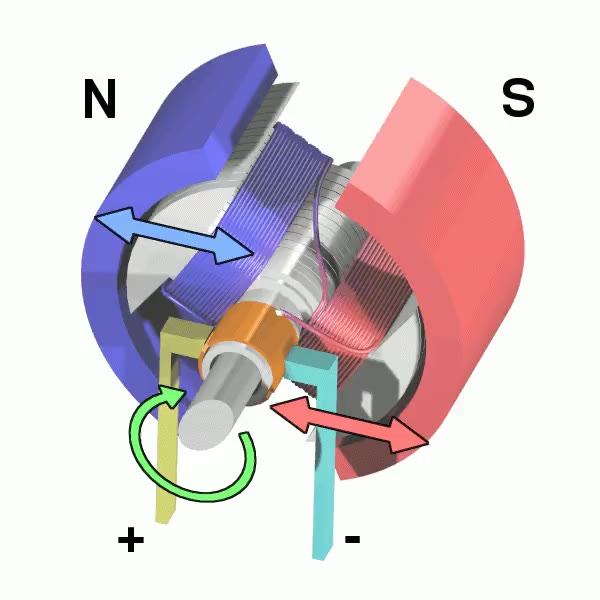
\includegraphics[width=0.2\columnwidth,valign=m]{images/dc_motor_3d_video.jpg}}{videos/dc_motor_3d.mp4}
        }
        \subfloat[]{
            \movie[autostart,poster,loop,showcontrols]{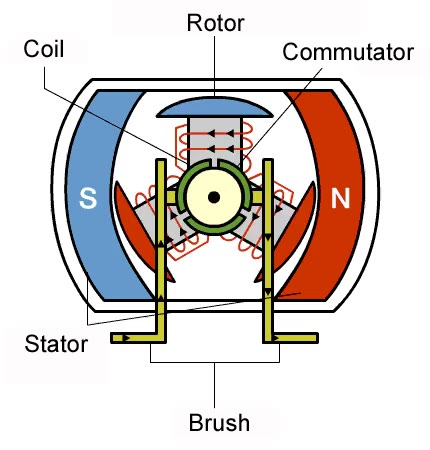
\includegraphics[width=0.2\columnwidth,valign=m]{images/dc_motor_video.jpg}}{videos/dc_motor.mp4}
        }
    \end{figure}
    
\end{frame}

\begin{frame}
    \frametitle{Controladores de Motores DC}
    \note{Información extraída de https://youtu.be/pEVsedl2KO4?si=_cwQpRPPUnQ04B3c}
    
    \begin{itemize}
        \item Más corriente = más rotación
        \item ¿Cómo modular corriente usando una señal digital?
        \item \emph{Pulse width modulation} (PWM)
        \item Duty cycle = ratio de tiempo vs periodo
    \end{itemize}
    
    \begin{figure}[!h]
        \subfloat[]{
            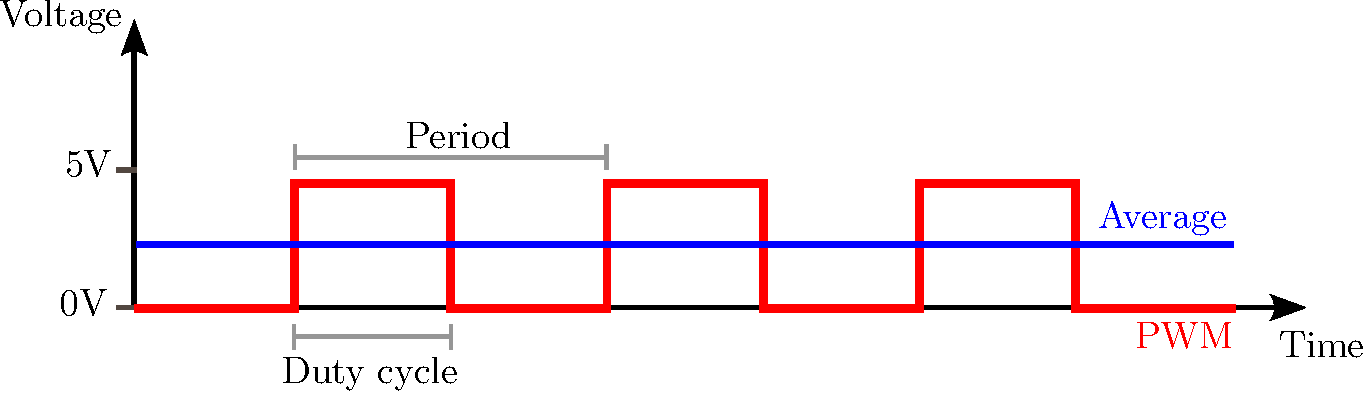
\includegraphics[width=0.6\columnwidth,valign=m]{images/pwm_signal.pdf}
        }
        \hfill
        \subfloat[]{
            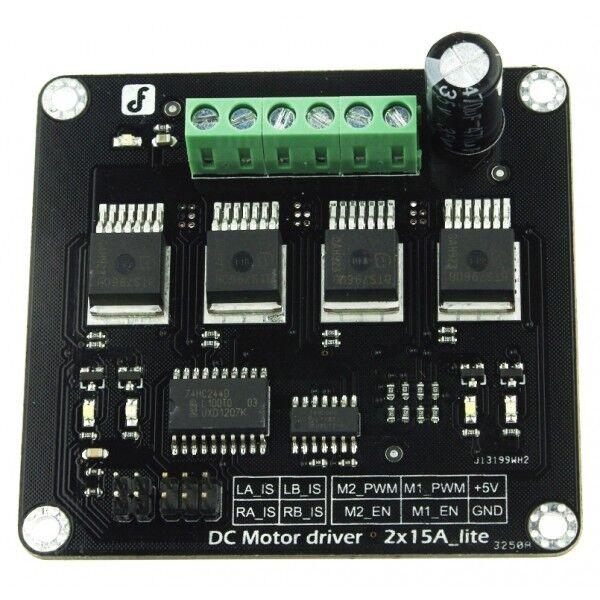
\includegraphics[width=0.3\columnwidth,valign=m]{images/dc_motor_driver_2x15A_lite.jpg}
        }
    \end{figure}
    
\end{frame}

\begin{frame}
    \frametitle{Open loop vs feedback control}
    \note{Información extraída de https://youtu.be/pEVsedl2KO4?si=_cwQpRPPUnQ04B3c}
    
    \begin{figure}[!h]
        \subfloat[Open loop control]{
            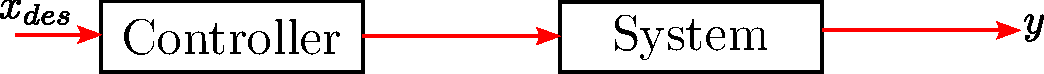
\includegraphics[width=0.6\columnwidth,valign=m]{images/open_loop_control.pdf}
        }
        
        \subfloat[Feedback control]{
            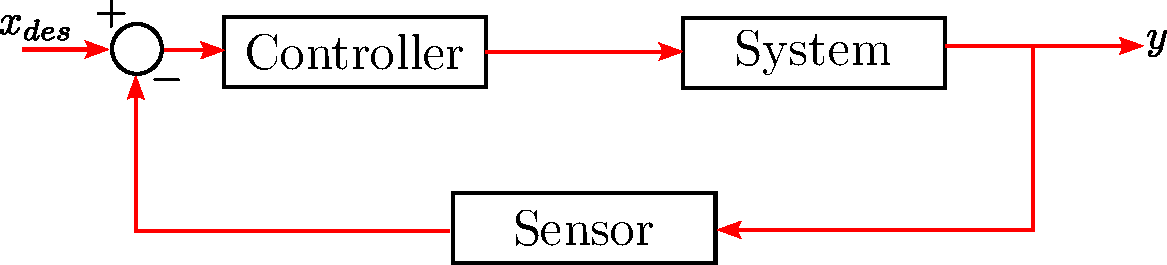
\includegraphics[width=0.7\columnwidth,valign=m]{images/feedback_control.pdf}
        }
    \end{figure}
    
\end{frame}

\begin{frame}
    \frametitle{Ejemplo de Feedback control}
    \note{Información extraída de https://youtu.be/pEVsedl2KO4?si=_cwQpRPPUnQ04B3c}
    
    \begin{center}
        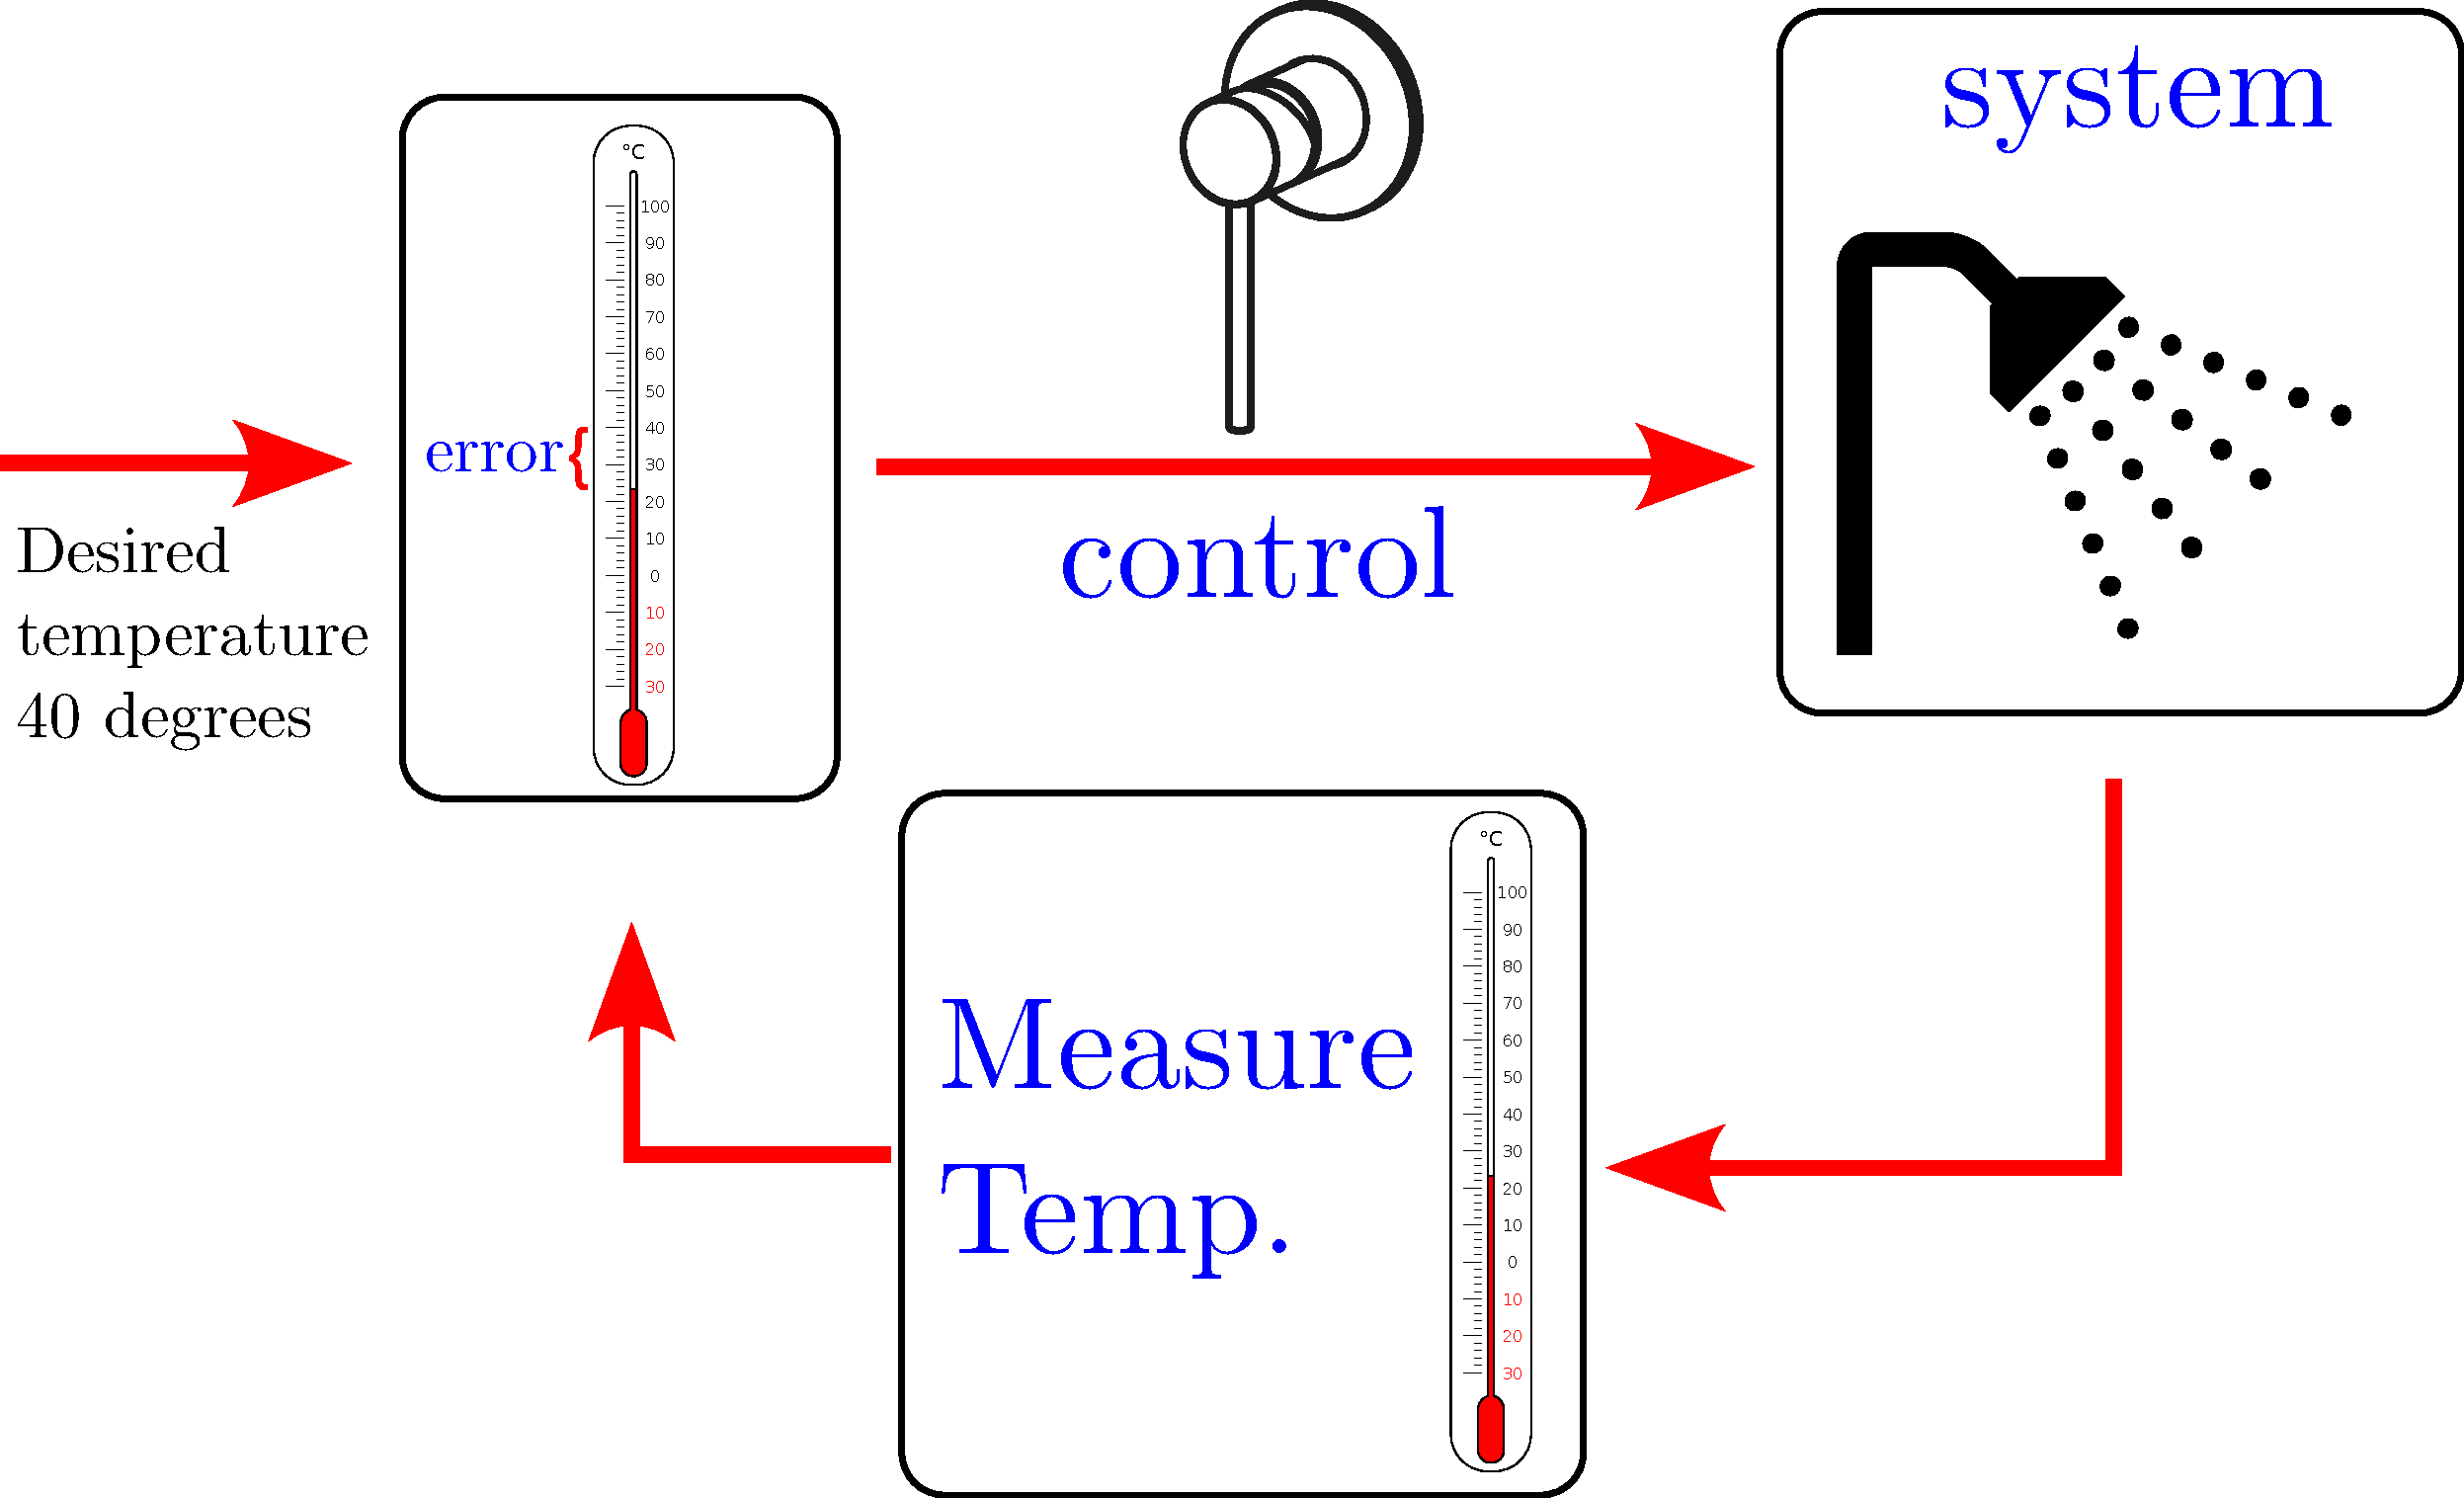
\includegraphics[width=0.6\columnwidth,valign=m]{images/temperature_feedback_control.pdf}
    \end{center}

    
\end{frame}

\begin{frame}
    \frametitle{Diagrama de bloques}
    \note{Información extraída de https://youtu.be/pEVsedl2KO4?si=_cwQpRPPUnQ04B3c}
    
    \begin{center}
        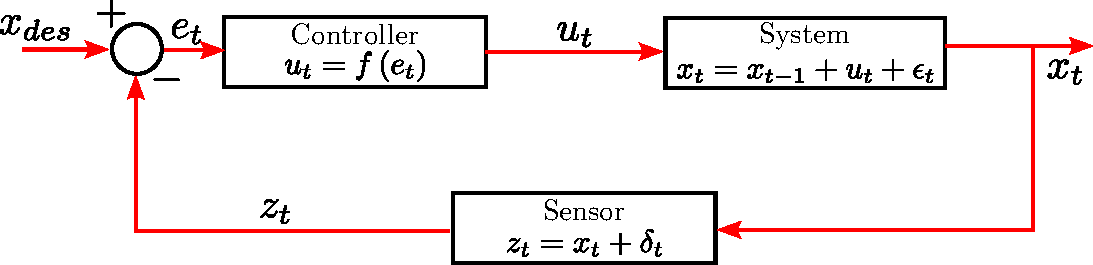
\includegraphics[width=0.8\columnwidth]{images/feedback_control_math.pdf}
    \end{center}
   
\end{frame}

\begin{frame}
    \frametitle{Proportional control}
    \note{Información extraída de https://youtu.be/pEVsedl2KO4?si=_cwQpRPPUnQ04B3c}
    
    \begin{itemize}
        \item P-Control: $\controlCommand_{t} = K_{p} e_{t}$ con  $K_{p} = 1$
    \end{itemize}
    
    \TODO{\url{https://www.zhinst.com/americas/de/resources/principles-of-pid-controllers}}
    
\end{frame}

\begin{frame}
    \frametitle{Motores DC}
    \note{Información extraída de https://youtu.be/pEVsedl2KO4?si=_cwQpRPPUnQ04B3c}
    
    \begin{itemize}
        \item 
    \end{itemize}
    
\end{frame}

\begin{frame}
    \frametitle{Motores DC}
    \note{Información extraída de https://youtu.be/pEVsedl2KO4?si=_cwQpRPPUnQ04B3c}
    
    \begin{itemize}
        \item 
    \end{itemize}
    
\end{frame}

\begin{frame}
    \frametitle{Motores DC}
    \note{Información extraída de https://youtu.be/pEVsedl2KO4?si=_cwQpRPPUnQ04B3c}
    
    \begin{itemize}
        \item 
    \end{itemize}
    
\end{frame}

\begin{frame}
    \frametitle{Motores DC}
    \note{Información extraída de https://youtu.be/pEVsedl2KO4?si=_cwQpRPPUnQ04B3c}
    
    \begin{itemize}
        \item 
    \end{itemize}
    
\end{frame}

\begin{frame}
    \frametitle{Motores DC}
    \note{Información extraída de https://youtu.be/pEVsedl2KO4?si=_cwQpRPPUnQ04B3c}
    
    \begin{itemize}
        \item 
    \end{itemize}
    
\end{frame}

\begin{frame}
    \frametitle{Motores DC}
    \note{Información extraída de https://youtu.be/pEVsedl2KO4?si=_cwQpRPPUnQ04B3c}
    
    \begin{itemize}
        \item 
    \end{itemize}
    
\end{frame}
